\documentclass[border=10pt]{standalone}
\usepackage[svgnames]{xcolor}
\usepackage{amsmath}
\usepackage{pgfplots}
\pgfplotsset{compat=newest}
\usepackage[sfdefault]{FiraSans}
\usepackage{FiraMono}
\renewcommand*\familydefault{\sfdefault}
\begin{document}
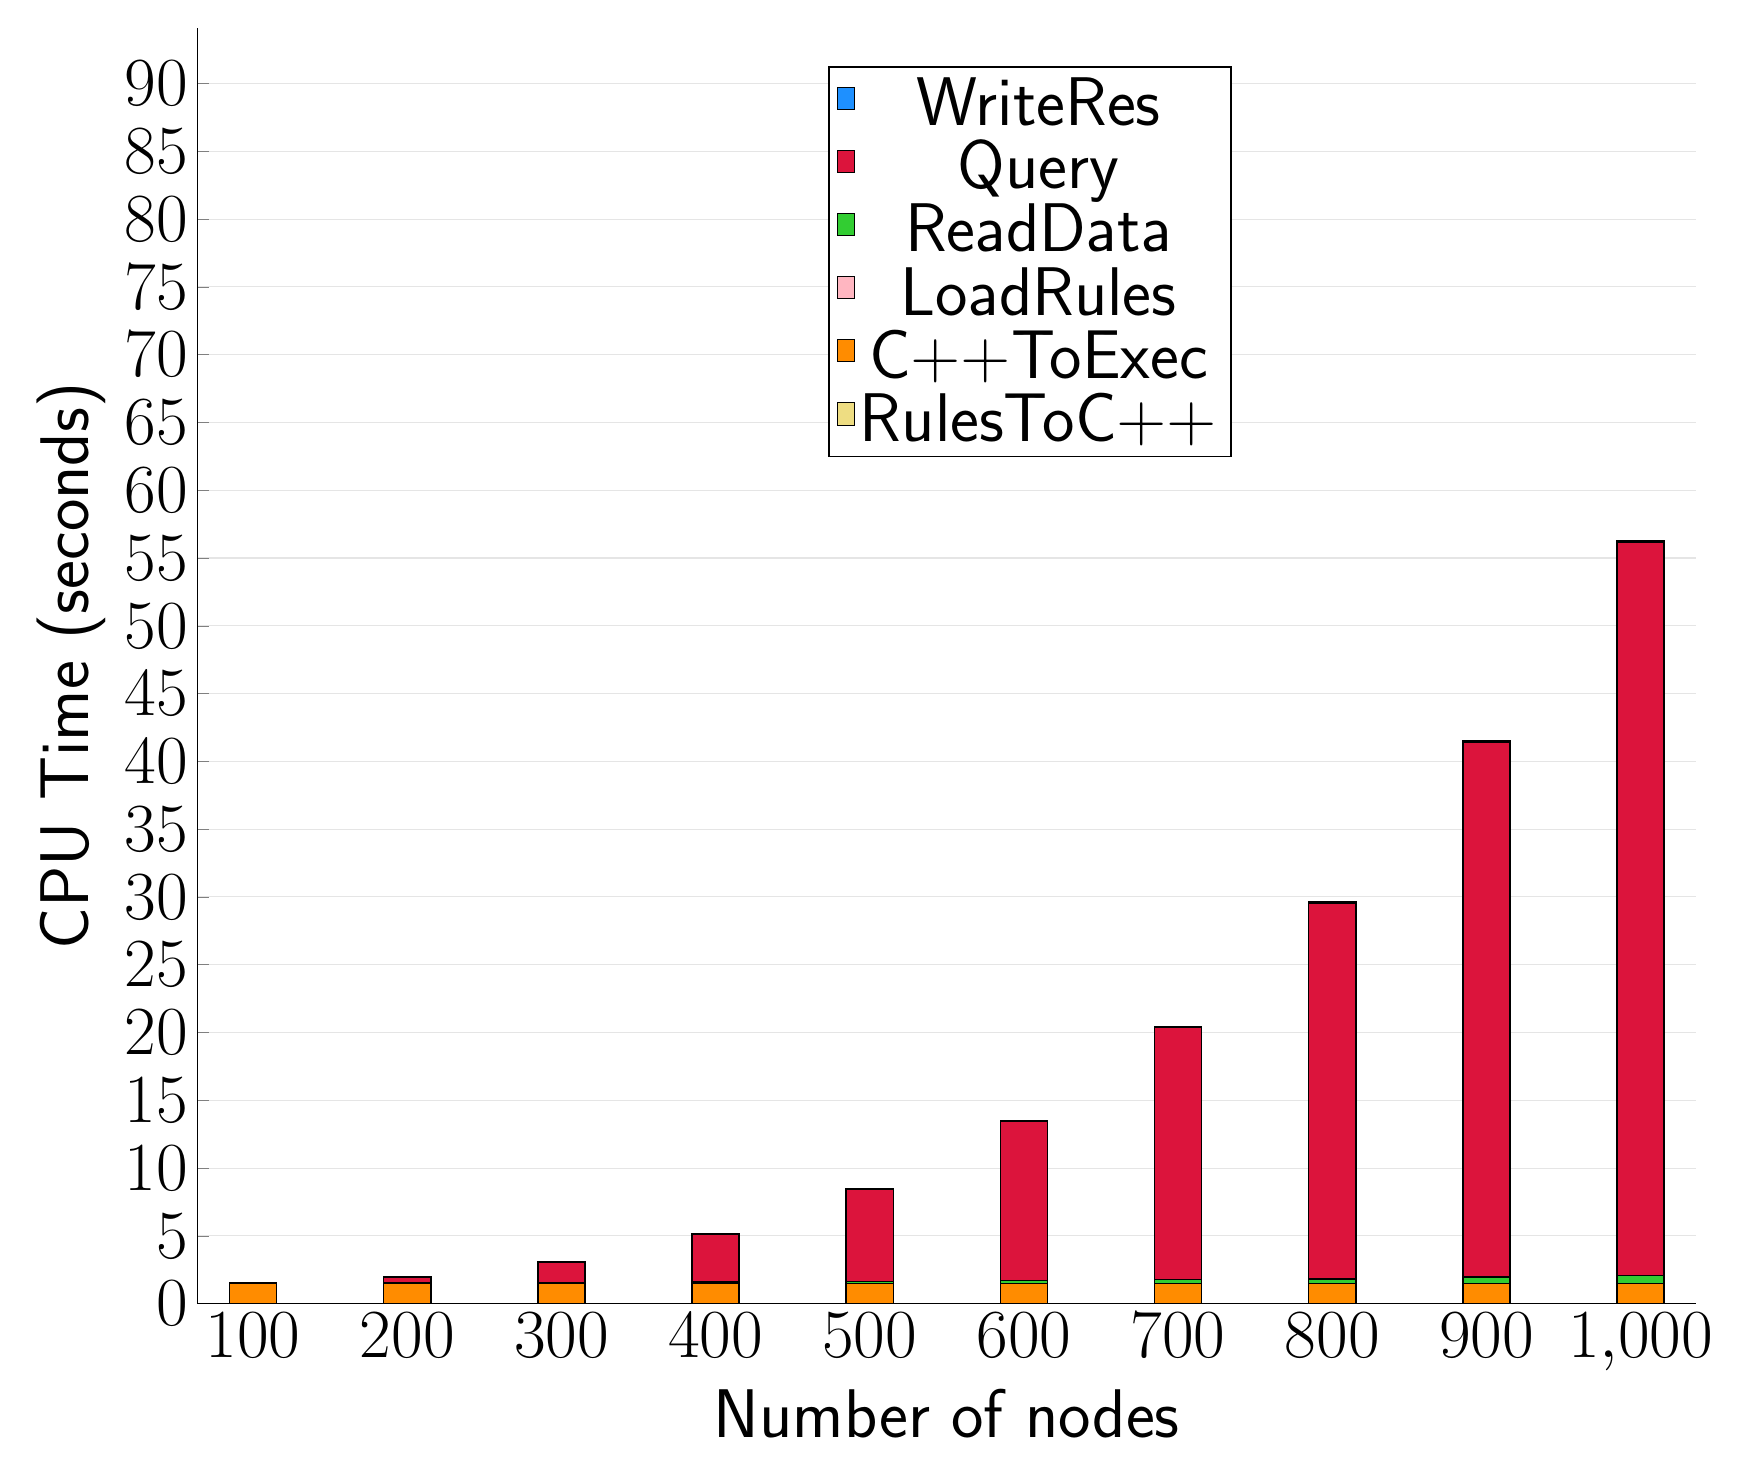
\begin{tikzpicture}
\begin{axis}[
   ybar stacked,
   width=1.7\textwidth,
   bar width=0.6cm,
   ymajorgrids, tick align=inside,
   major grid style={draw=gray!20},
   xtick=data,
   ymin=0, ymax=94.08204,
   axis x line*=bottom,
   axis y line*=left,
   enlarge x limits=0.04,
   legend style={
       at={(0.69, 0.97)},
       anchor=north east,
       legend columns=1,
       font=\Huge,
   },
   ylabel={CPU Time (seconds)},
   xlabel={Number of nodes},
   label style={font=\Huge},
   tick label style={font=\Huge},
]
\addlegendimage{fill=DodgerBlue, draw=black, line width=0.2pt}
\addlegendentry{WriteRes}
\addlegendimage{fill=Crimson, draw=black, line width=0.2pt}
\addlegendentry{Query}
\addlegendimage{fill=LimeGreen, draw=black, line width=0.2pt}
\addlegendentry{ReadData}
\addlegendimage{fill=LightPink, draw=black, line width=0.2pt}
\addlegendentry{LoadRules}
\addlegendimage{fill=DarkOrange, draw=black, line width=0.2pt}
\addlegendentry{C++ToExec}
\addlegendimage{fill=LightGoldenrod, draw=black, line width=0.2pt}
\addlegendentry{RulesToC++}
\addplot +[fill=LightGoldenrod, draw=black, line width=0.55pt] coordinates {
(100, 0.004000000000000001)
(200, 0.006000000000000001)
(300, 0.006000000000000001)
(400, 0.008000000000000002)
(500, 0.004000000000000001)
(600, 0.0020000000000000005)
(700, 0.0)
(800, 0.008000000000000002)
(900, 0.0)
(1000, 0.0020000000000000005)
};
\addplot +[fill=DarkOrange, draw=black, line width=0.55pt] coordinates {
(100, 1.4740000000000002)
(200, 1.472)
(300, 1.472)
(400, 1.468)
(500, 1.468)
(600, 1.478)
(700, 1.4739999999999998)
(800, 1.462)
(900, 1.4759999999999998)
(1000, 1.484)
};
\addplot +[fill=LightPink, draw=black, line width=0.55pt] coordinates {
(100, 0.0001826)
(200, 0.0001764)
(300, 0.0001784)
(400, 0.00018159999999999997)
(500, 0.00018699999999999996)
(600, 0.0001858)
(700, 0.0001928)
(800, 6.88e-05)
(900, 0.0001724)
(1000, 0.0001852)
};
\addplot +[fill=LimeGreen, draw=black, line width=0.55pt] coordinates {
(100, 0.0147196)
(200, 0.0414628)
(300, 0.0742898)
(400, 0.1140728)
(500, 0.16531060000000003)
(600, 0.22715000000000002)
(700, 0.30176220000000004)
(800, 0.364879)
(900, 0.4838433999999999)
(1000, 0.59645)
};
\addplot +[fill=Crimson, draw=black, line width=0.55pt] coordinates {
(100, 0.07268300000000001)
(200, 0.45013900000000007)
(300, 1.492988)
(400, 3.5092559999999997)
(500, 6.8185720000000005)
(600, 11.748740000000002)
(700, 18.58492)
(800, 27.73096)
(900, 39.44554)
(1000, 54.082040000000006)
};
\addplot +[fill=DodgerBlue, draw=black, line width=0.55pt] coordinates {
(100, 0.0012812000000000001)
(200, 0.0045504000000000005)
(300, 0.0101084)
(400, 0.0173686)
(500, 0.027021800000000002)
(600, 0.0398912)
(700, 0.0522274)
(800, 0.0686598)
(900, 0.0868878)
(1000, 0.1058422)
};
\end{axis}
\end{tikzpicture}

\end{document}
